\documentclass{article}



\usepackage{arxiv}

\usepackage[utf8]{inputenc} % allow utf-8 input
\usepackage[T1]{fontenc}    % use 8-bit T1 fonts
\usepackage{hyperref}       % hyperlinks
\usepackage{url}            % simple URL typesetting
\usepackage{booktabs}       % professional-quality tables
\usepackage{amsfonts}       % blackboard math symbols
\usepackage{nicefrac}       % compact symbols for 1/2, etc.
\usepackage{microtype}      % microtypography
\usepackage{lipsum}		% Can be removed after putting your text content
\usepackage{graphicx}
\usepackage{natbib}
\usepackage{doi}
\usepackage{amsmath,amsfonts,amssymb,amsthm}
\usepackage{enumitem}
\usepackage{adjustbox}
\usepackage{array,ragged2e}
\usepackage{longtable}
\usepackage{pdflscape}
\usepackage{makecell}
\usepackage[font=small]{caption}
\usepackage[justification=centering]{caption}
\usepackage{booktabs}
\usepackage{chngcntr} % for local labelling
\usepackage{mathtools, nccmath}
\usepackage{physics}
\usepackage{subfig}
\usepackage{fancyvrb}
\usepackage{tcolorbox} % Grey Box Hightlight
\usepackage{color}
\usepackage{float}
\usepackage[fontsize=12pt]{fontsize}
\setlength\parindent{0pt}


\graphicspath{{../images/}} % NOTE: Put all your figures in this directory.

\title{Final Report for Independent Study In P300 Spellers: Understanding the Subject Progress and Investigating Some Representative Solutions}

\author{
	Zion Sheng (NetID: zs144)\\
	Department of ECE, Duke University\\
	Durham, NC 27708 \\
	\texttt{zion.sheng@duke.edu} \\
}

\date{} % remove the date

% Uncomment to override  the `A preprint' in the header
% \renewcommand{\headeright}{Technical Report}
\renewcommand{\undertitle}{Supervisor: Prof. Leslie Collins, Prof. Boyla Mainsah}
% \renewcommand{\shorttitle}{\textit{arXiv} Template}

%%% Add PDF metadata to help others organize their library
%%% Once the PDF is generated, you can check the metadata with
%%% $ pdfinfo template.pdf
\hypersetup{
	pdftitle={A template for the arxiv style},
	pdfsubject={machine learning},
	pdfauthor={Zion Sheng},
	pdfkeywords={EEG signal processing, brain-computer interface, P300 speller, machine learning, convolutional neural network, n-gram language model},
}

\begin{document}
\maketitle

\vspace{-10mm}
\begin{abstract}
	Brain-computer interface (BCI) is a broad collection of machines that can facilitate the interaction between human brains and external devices. Generally, each type of BCI is designed to work on a specific task, where the P300 speller can help users in spelling. By classifying whether received electroencephalogram (EEG) signals contain a special event-related potentials (ERP) called P300, it can infer the user's desired character. Among all the traditional classification algorithms, stepwise linear discriminant analysis (SWLDA) reaches the state-of-the-art performance, and it can be further enhanced by some language models. Nevertheless, with the emergence of many powerful deep learning techniques, recent studies have turned to exploring the applications of deep neural networks on P300 spellers. This report tries to deliver a concise overview of the freshly-finished independent study. It will start from the problem description and subject progress, and then proceed to elaborate on the two competitive solutions: one is SWLDA combined with an 2-gram language model, and the other is EEGNet, a convolutional neural network tailored for P300 BCIs. The two methods are implemented and tested on the real data from 17 participants. Results demonstrate that EEGNet has better generalizability that is unprecedented in SWLDA, but the latter still achieves a higher spelling accuracy on average.
\end{abstract}


% keywords can be removed
\keywords{EEG signal processing, brain-computer interface, P300 speller, machine learning}


\section{Introduction} \label{Description}
\subsection{Background} \label{Background}
Recently, Brain-computer interfaces (BCIs) have gained increasing attention as an alternative human-machine communication tool. Many BCIs are reported to have the potential to augment normal people's perception ability and extend physical limits. But more importantly, many BCIs can help to restore control/communication ability and mobility to disabled people. Among these types of BCIs, the P300 speller is targeted at individuals with severe neuromuscular injuries who can not communicate effectively by speaking, writing, or typing in a regular manner. Typical users of P300 spellers are Amyotrophic lateral sclerosis (ALS) patients, especially in the late stage of the disease (commonly known as the "locked-in" stage) as the nervous system has lost most muscle control \cite{moghimi2013review}. These patients cannot move any part of their body, including vocal cords, fingers, and eyes, to complete even a simple spelling task in any language. However, as long as the brain and cognitive ability are in normal operation, there is still hope. The first P300 speller was created by \cite{farwell1988talking}, which enables the user to "type" on a virtual keyboard on the screen by utilizing a special EEG signal called the P300 waves. Based on this pioneering work, later scientists proposed many new designs by applying better hardware, improving the inner algorithms, and adapting the display settings, but the general framework of the P300 spellers didn't change much.\\

\vspace{-3mm}
Before starting to elaborate on the general framework, it is necessary to give a brief explanation of what is the P300 wave and why it can be used on these machine-assisting spelling tasks. The fundamental biological principle behind all BCI is that the brain (or generally, the neural system) generates electrical signals/waves along with all kinds of neural activities, where different stimuli (inputs) and intended reactions (outputs) will lead to various responses, i.e., different shapes of the signals/waves. These signals/waves depending on the preceding events are called event-related potentials (ERPs), and the P300 waves also fall in this category. The P300 waves occur due to a ubiquitous neural activity mechanism called the oddball paradigm, which happens when the subject detects the appearance of a rare stimulus (target) out of some common stimulus (non-targets) presented more frequently. Such a mechanism will lead to two different brainwaves depending on the type of the received stimuli. Figure \ref{fig:1} illustrates a representative waveform of the P300 wave (red line) VS non-P300 wave using the data from one of the participants in the experiment. More details about the data will be given in the later sections, but the visualization here is already sufficient to pass the intuition that the P300 wave is distinguishable from non-P300 wave as there is a positive deflection in voltage occurs around 200 ms - 400 ms after the target stimulus is presented (when \texttt{Time = 0s}), while the non-P300 waves remain regular after the non-target stimulus onset.

\vspace{-3mm}
\begin{figure}[H]
	\centering
	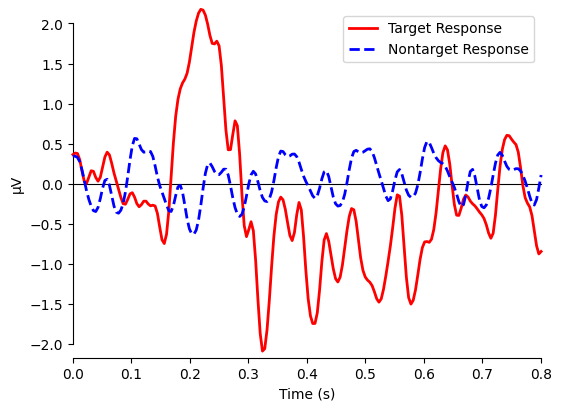
\includegraphics[width=0.5\linewidth]{waves.png}
	\vspace*{-1.5mm}
	\captionof{figure}{Waveforms of P300 waves (elicited by target stimuli) and non-P300 waves}
	\label{fig:1}
\end{figure}

\vspace{-3mm}
This useful mechanism can be applied to the settings of the visual display of a keyboard, commonly used as the interface of the P300 speller. Subjects are asked to focus on their desired character on the keyboard (only one at a time) when a random subset of these characters gets flashed every time. Suppose there are $N$ characters in total and the subset size is $k$, then the probability of the target being flashed is around ${N \choose k-1} / {N \choose k} = \frac{k}{N-k+1}$. Therefore, such a rare event can elicit a P300 wave every time it happens. Theoretically, the desired character should be the one eliciting the most number of P300 waves, so the P300 speller can infer it after a certain amount of flashes.

\subsection{General Framework of P300 spellers} \label{Framework}
There are three key components in the general framework that apply to every P300 speller: a screen to show the keyboard, a headset to collect EEG signals, and a computer to serve the communication between subjects and the keyboard. The connection of these components is shown in Figure \ref{fig:2}.

\vspace{-3mm}
\begin{figure}[H]
	\centering
	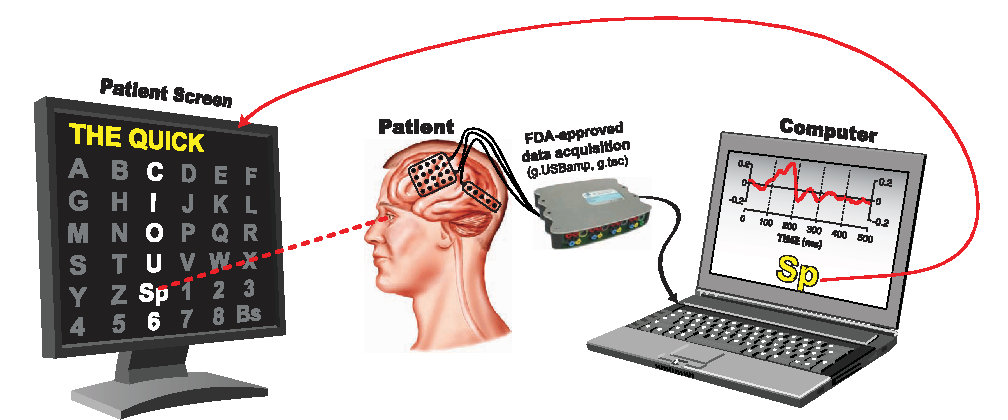
\includegraphics[width=0.7\linewidth]{overview.png}
	\captionof{figure}{The general framework of P300 spellers (credit: \cite{brunner2011rapid})}
	\label{fig:2}
\end{figure}

\vspace{-3mm}
The general process is that, the computer first acts as the scheduler of the character display by picking a subset of characters to flash every round with a fixed time interval. There are several popular flashing paradigms, and in our experiment, we choose the "RC" (row-column) paradigm, which flashes a whole row or column in each round. Users are asked to focus on the desired character and count how many times it gets flashed. By doing so, the P300 wave will be generated once the targeted character is in the flashed row or column. Users also need to wear a headset to monitor the EEG signals from different areas on the brain surface. These sensors are not invasive, and we can only collect signals from certain areas where the signals are strong, although the noise in data still needs further processing. Next, the data will be transmitted to the computer where a pre-trained user-specific classifier is deployed to decide whether a P300 wave occurs. The computer will keep track of the decisions and accumulate them as a score for each character. Once it is confident to infer the desired character, it will spell it on the screen, marking the end of a cycle. By repeating the above steps, users can spell a complete word or sentence. The inference tends to be more accurate with more flashes (or called "trials"), but the side-effect is that users will gradually get bored and distracted. Clearly, there is a trade-off between the inference accuracy and efficiency. Another concern is that every row and column should be flashed by the same amount of times to avoid any unfairness, so the total flashes to spell one character are usually measured as $s$ sequences, where one sequence is flashing all rows and columns once.


\subsection{Our work} \label{Work}
Based on this basic framework, there are many flexibilities in the actual design. Past studies have extended and upgraded the P300 spellers from the very first one (\cite{farwell1988talking}) to a huge family where each member has some valuable features. \cite{elshout2009review} and \cite{fang2021recent} respectively provide a comprehensive review on the progress of P300 spellers. By learning this history, we can see the evolutional path of the improvements in hardware, in displaying settings, and especially in classification and inference algorithms since the emergence of deep learning-based techniques in the last decade. Serving as the final report for this independent study, we will specifically focus on two representative P300 spellers in history. They are different in the choice of signal-classification and character-inference algorithms, but both are reported to achieve a competitive performance. One of them uses step-wise linear discriminant analysis (SWLDA) combined with Bayesian inference, whereas another one is powered by a convolutional neural network (called EEGNet) with simple counting. The first one is the generative probabilistic model as we need to estimate the conditional distribution of the target class and non-target class. On the contrary, the second one is essentially a discriminative neural network since it only outputs the decision results. In addition, it is also worth mentioning that the first one can be further enhanced using a 2-gram language model to utilize the previously spelled character. We will elucidate all these technical details in the following sections.\\

\vspace{-3mm}
In this report, we first go through the related papers to figure out the details of the two methods, which will be covered in Section \ref{Methods}. Then, we implemented the algorithmic part of the two methods in Python and tested them on the dataset we borrowed from \cite{mainsah2014utilizing} (we received the permission of the original authors). The specifications of the data and experiment setup are clearly explained in Section \ref{Experiment}. Results are provided in Section \ref{Results}, where we also included the supplementary analysis by comparing the two methods and their variations qualitatively and quantitatively. Finally, \ref{Conclusion} gives a brief summary of this independent study accompanied by some thoughts for future work.


\section{Methods} \label{Methods}
First, let's take a quick look at the workflow of the algorithmic part of P300 spellers as shown in Figure \ref{fig:3}. The gray boxes (steps) are shared commonly in both methods, whereas the red boxes indicate the places to make different design choices. 

\vspace{-3mm}
\begin{figure}[H]
	\centering
	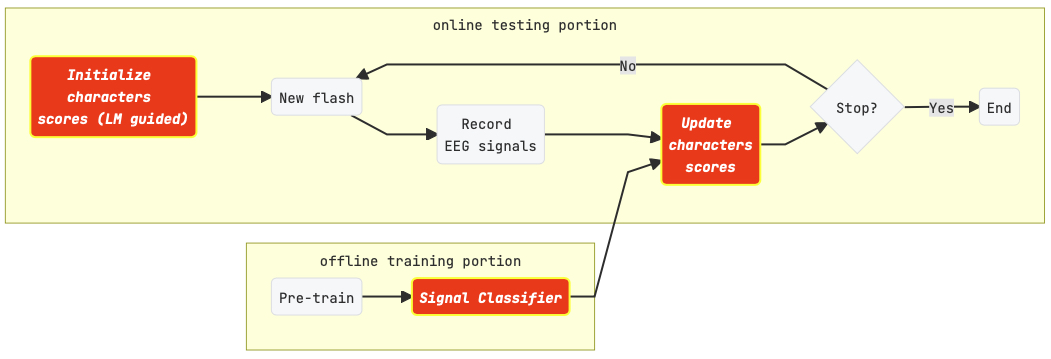
\includegraphics[width=1.0\linewidth]{framework.jpg}
	\captionof{figure}{The general workflow of the algorithmic part of P300 spellers}
	\label{fig:3}
\end{figure}

\vspace{-3mm}
We start from the offline training portion in the lower part of Figure \ref{fig:3}. Here, we need to pre-train a classifier so that it can detect the presentation of the P300 signal given a standardized chunk of EEG wave which usually span from the beginning of the stimulus onset till $800$ ms later. Due to the high variance of the reactions from different subjects to the same stimuli, traditionally it is recommended to train a signal classifier for each user based on his/her training data. However, recent DL-based methods suggest a robust generalizability can be achieved. Therefore, we will stick to the traditional approach when training the SWLDA classifier, and for EEGNet, we will try to build a general classifier without being user-specific. Now, we are ready to move on to the online experiment portion, where "online" refers to the real-time application of the P300 speller. To spell each letter, the computer first needs to initialize the character scores. The initial scores are the same, but as we start the iterations of the flash and update, the scores will change and polarize. In each iteration, we will randomly choose a row and column to flash. The subject is required to focus on the desired character and count the times it gets flashed. The observation of the EEG signal in a fixed time interval (800 ms) is sent to the classifier in the computer and the output is returned to update the scores. The general rule is that characters in any row or column that elicits a P300 wave should have a higher score increment. Theoretically, only the row and the column where the desired character resides can generate a P300 signal, so the score of that character should be the highest after some trials.\\

\vspace{-3mm}
However, in practice, the EEG signals we collect are very noisy, making the classifier prone to make a wrong classification. This can severely disturb the inference of the target. Thus, we need to either find a better classification algorithm that can survive under a low signal-to-noise (SNR) ratio, OR we can try to avoid the erroneous tendency by some special processing, such as applying some language model when initializing the scores (as we highlighted in the top-left box of Figure \ref{fig:3}). Even though the subject can only spell a single character each time, those previously typed ones can still provide useful information.



\subsection{Methods 1: SWLDA + Bayesain Inference (enhanced by the Language Model)} \label{SWLDA}
This approach uses SWLDA as the signal-classification algorithm (the red box in the bottom of Figure \ref{fig:3}), Bayesian inference as the score-updating algorithm (the red box in the middle-left of Figure \ref{fig:3}), and the 2-gram LM to aid the score initialization (the red box in the top-left of Figure \ref{fig:3}). We have learned LDA in class. Recall that LDA aims to find a linear combination of features that can maximize the separation of different classes while maintaining a low variance within each class. SWLDA is essentially LDA but trained in a stepwise manner. In each iteration, SWLDA will try different combinations by adding or dropping some features based on certain criteria until it finally finds the optimal one. To implement SWLDA, we refer to the existing \texttt{stepwisefit} function in \texttt{MATLAB} and LDA implementation in \texttt{Scikit-learn}, the code is enclosed in \texttt{swlda.py} submitted with this report.\\

\vspace{-3mm}
Now suppose the classifier is well-trained and can correctly return the classification score for every EEG input data, now we need to think about how to update the score of each character. Bayesian inference uses the Bayes theorem to update the probability of each character being the target given the information accumulated along the trails. To do this, we need to estimate the probability density function of the classifier scores ($y$) of non-P300 waves (non-target) and P300 waves (target), defined as $P(y|H_0)$ and $P(y|H_1)$ respectively. Let $C_m$ denote any character, and $C^*$ denote the target character. From trail $0$ to trail $t$, suppose $\boldsymbol{F_t}=[\mathcal{F}_1, \mathcal{F}_2, ..., \mathcal{F}_t]$ is a series of stimulus event presentations, and $\mathbf{Y_t} = [y_1, y_2, ..., y_t]$ is classifier score responses. After each stimulus is presented, the classifier score, $y_t$, will be used to update the character probabilities:

\begin{equation} \label{eq:1}
	P(C_m = C^*|\mathbf{Y_t}, \mathcal{F}_t) = \frac{P(C_m = C^*|\mathbf{Y_{t-1}}, \mathcal{F}_{t-1})p(y_t|C_m = C^*, \mathcal{F}_t)}{\sum^M_{j=1}P(C_j = C^*|\mathbf{Y_{t-1}}, \mathcal{F}_{t-1})p(y_t|C_j = C^*, \mathcal{F}_t)}
\end{equation}

The likelihood, $p(y_t|C_m = C^*, \mathcal{F}_t)$, for each character $C_m$ is updated depending on whether or not the character is in the flashed subset:

\begin{equation} \label{eq:2}
	p(y_t|C_m = C^*, \mathcal{F}_t) = \left\{
	\begin{aligned}
		& p(y_t|H_0) & (C_m \notin \mathcal{F}_t) \\
		& p(y_t|H_1) & (C_m \in \mathcal{F}_t) \\
	\end{aligned} 
\right.
\end{equation}

The final thing that needs to be specified is the initial probability score of each character, denoted by $P(C_m = C^*|\mathbf{Y_0}, \mathcal{F}_0)$. An intuitive way is to set them all equally to $1/N$ where $N$ is the number of characters. This works well for the first letter to spell, but for the later letters, it's not the most effective way since we waste the information from the previously typed letters. Typically, subjects are required to type a meaningful English word (usually contains 5-7 letters). Given the prior knowledge of the first few letters, the probability distribution of letters in the current location is not uniform. Now suppose any English word can be decomposed into a series of characters $[c_1, c_2, ..., c_k]$. Here, we are going to apply a 2-gram model to correct the initial probability scores for the second and following letters. Firstly, we approximate the conditional probabilities $P(c_i|c_{i-1})$ by maximum likelihood estimation using a relative frequency count $f(c_{i-1}c_{i})$ and $f(c_{i-1})$. Then, the conditional probability of choosing character $c_i$ given the previous one being $c_{i-1}$ will be:

\begin{equation} \label{eq:3}
	P(c_i|c_{i-1}) = \frac{f(c_{i-1}c_{i})}{f(c_{i-1})}
\end{equation}
	
As \cite{mainsah2014utilizing} suggests, we choose to use the Carnegie Mellon University online dictionary as the training corpus to derive the conditional probabilities. The result can be visualized by the paired probability matrix shown in Figure \ref{fig:4} below:

\vspace{-3mm}
\begin{figure}[H]
	\centering
	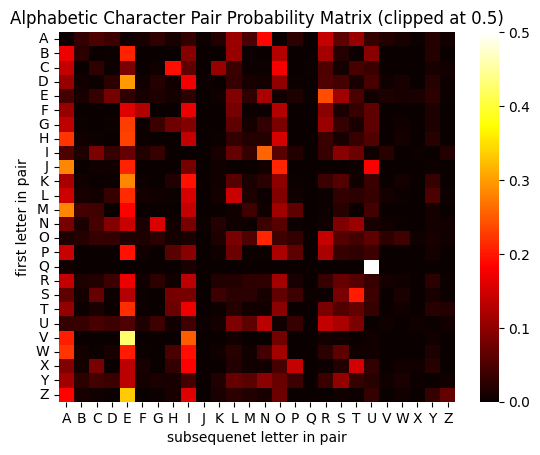
\includegraphics[width=0.5\linewidth]{2gram.png}
	\captionof{figure}{Probability matrix of paired English character}
	\label{fig:4}
\end{figure}

\vspace{-3mm}
Before we integrate the language model with the rest of the algorithmic part, we need to address the concern that the previously typed letter is incorrect. To avoid the possible negative effect, we can neutralize the LM-guided probability distribution with the uniform distribution we used before. Another detail that needs to be taken care of is that not all characters on the keyboard are English letters, so we need to rescale the probability. The final form of the equation to initialize the probability scores of the $n$-th character can be expressed by:

\begin{equation} \label{eq:4}
	P(C_i) = \alpha P(C_i|A_{i-1})(1 - \frac{m}{N}) + (1-\alpha)\frac{1}{N}
\end{equation}

where $P(C_i|A_{i-1})$ denotes the initial probability of each character being the target given that the previous letter is letter $A_{i-1}$, which can be found in the probability matrix in Figure \ref{fig:4}. Finally, $\alpha$ is set to $0.9$ since it is proved to work well on simulations in \cite{mainsah2014utilizing}.


\subsection{Methods 2: EEGNet + Simple Counting} \label{EEGNet}
As the competitor of the above approach, Method 2 utilizes a neural network called EEGNet introduced by \cite{lawhern2018eegnet} to detect the target signals. This network has been verified to work well on many EEG-related problems, including the P300 speller (\cite{lee2020cnn}). Figure \ref{fig:5} shows the general architecture of the EEGNet. Different from SWLDA, EEGNet consumes the data of all users as the training input. The training data is concatenated together with each column representing a timestamp (spanning from $0$ to $800$ ms) and each row recording the EEG signal of a certain subject at a certain trail. The input first is processed by a 2D convolutional layer, which extracts the temporal features of the signals. Then, the output feature map is passed to a 2D depthwise convolutional layer, where the spatial features in each feature map are learned. Next, the third layer is a combination of multiple depthwise convolutional layers, which serve to summarize the temporal information in each feature map respectively. Finally, the output will be processed by a pointwise convolutional layer to further synthesize the feature information and make the final classification decision.

\begin{figure}[H]
	\centering
	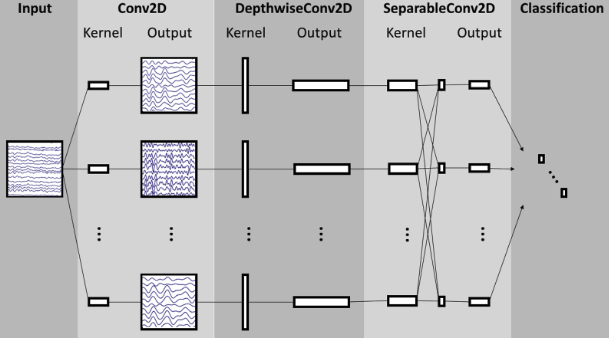
\includegraphics[width=0.7\linewidth]{architecture.jpg}
	\captionof{figure}{General architecture of EEGNet (Credit: \cite{lawhern2018eegnet})}
	\label{fig:5}
\end{figure}

\vspace{-3mm}
Depending on the input size, the size of kernels in EEGNet should be adapted correspondingly. Following the instruction in \cite{lawhern2018eegnet} and the actual input data size in our experiment (see Section \ref{Data}), we designed our EEGNet and implemented it by \texttt{PyTorch}. The code will be publicized in the GitHub repository later. Figure \ref{fig:6} summarizes the detailed information about the model structure, where each "Sequential" from top to bottom corresponds to the convolutional layer from left to right. The final Linear layer is the classification layer at the rightmost of Figure \ref{fig:5}.

\begin{figure}[H]
\scriptsize
\centering
\begin{BVerbatim}
	==========================================================================================
	Layer (type:depth-idx)                   Output Shape              Param #
	==========================================================================================
	EEGNet                                   [4284, 2]                 --
	+-Sequential: 1-1                        [4284, 64, 32, 207]       --
	|    |-Conv2d: 2-1                       [4284, 64, 32, 207]       4,096
	|    |-BatchNorm2d: 2-2                  [4284, 64, 32, 207]       128
	+-Sequential: 1-2                        [4284, 256, 1, 51]        --
	|    |-Conv2d: 2-3                       [4284, 256, 1, 207]       8,192
	|    |-BatchNorm2d: 2-4                  [4284, 256, 1, 207]       512
	|    |-ELU: 2-5                          [4284, 256, 1, 207]       --
	|    |-AvgPool2d: 2-6                    [4284, 256, 1, 51]        --
	|    |-Dropout: 2-7                      [4284, 256, 1, 51]        --
	+-Sequential: 1-3                        [4284, 256, 1, 6]         --
	|    |-Conv2d: 2-8                       [4284, 256, 1, 52]        4,096
	|    |-Conv2d: 2-9                       [4284, 256, 1, 52]        65,536
	|    |-BatchNorm2d: 2-10                 [4284, 256, 1, 52]        512
	|    |-ELU: 2-11                         [4284, 256, 1, 52]        --
	|    |-AvgPool2d: 2-12                   [4284, 256, 1, 6]         --
	|    |-Dropout: 2-13                     [4284, 256, 1, 6]         --
	+-Linear: 1-4                            [4284, 2]                 3,074
	==========================================================================================
	Total params: 86,146
	Trainable params: 86,146
	Non-trainable params: 0
	Total mult-adds (Units.GIGABYTES): 139.03
	==========================================================================================
	Input size (MB): 112.96
	Forward/backward pass size (MB): 34059.31
	Params size (MB): 0.34
	Estimated Total Size (MB): 34172.61
	==========================================================================================
\end{BVerbatim}
\caption{The information summary of each layer in our EEGNet}
\label{fig:6}
\end{figure}

\vspace{-3mm}
Since this EEGNet classifier is essentially a discriminative model, it can not directly work with the Bayesian inference algorithm we used before. Instead, we choose to count the number of times each character is classified as the target. In other words, if the character is in the row or column which is classified as eliciting a P300 wave, it will be incremented by 1. Otherwise, the score remains unchanged. In this way, there is no probabilistic method included here. It is still possible to adapt the language model to carry on the information of prior letters, but it is unknown what value we should assign at the beginning. Therefore, we decide to abandon the language model in this case and initialize all the scores to $0$.

\section{Experiment} \label{Experiment}
\subsection{Data} \label{Data}
The data we used is borrowed from \cite{mainsah2014utilizing} as we are granted permission by the original authors Prof. Mainsah and Prof. Collins at Duke University. The original studies were approved and financed by Duke University and East Tennessee State University. For the hardware side, the study used 32-channel electrode caps to collect the EEG data, and the open-sourced BCI2000 software suite to process the signals. The distribution of the electrode is visualized in Figure \ref{fig:7} (a). Also, the keyboard (see Figure \ref{fig:7} (b)) used by the study is a standard $8 \times 9$ keyword adopted commonly in many P300 speller research.

\vspace{-3mm}
\begin{figure}[H]
	\centering
	\subfloat[\centering Brainmap of the headset electrodes]
	{{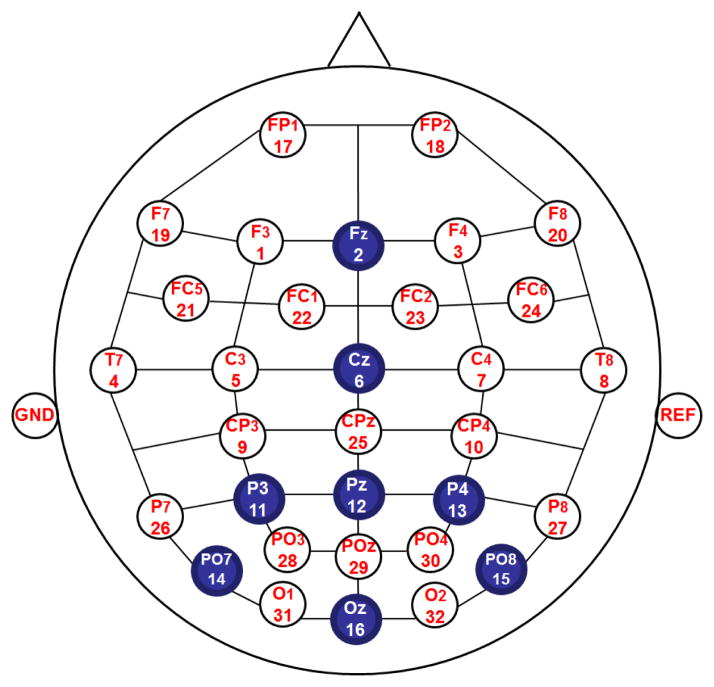
\includegraphics[width=6.5cm]{brainmap.jpg} }}%
	\qquad
	\hspace{-8mm}
	\subfloat[\centering Keyboard]
	{{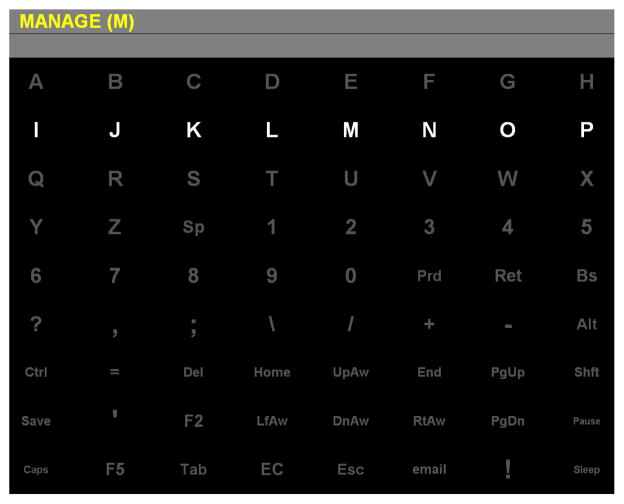
\includegraphics[width=6.5cm]{keyboard.jpg} }}%
	\caption{Visual display of some hardware used in the experiment}
	\label{fig:7}
\end{figure}

\vspace{-3mm}
In our study, we chose to use the data from the 13 participants since there is some missing data in the other 6 participants. Each one is required to complete one training section and one testing section. In every section, participants are required to type 5 "words" (some words contain non-alphabetic characters), with a total number of 36 characters. To spell each character, participants need to go through 7 sequences, i.e., $7 \times (8 + 9) = 119$ trails. Thus, each one will generate $119 \times 36 = 4289$ trials for a training section or a testing section. Now let's look closely at each trial. There are 32 electrodes working to collect EEG signals at different locations simultaneously. The frequency is 256 Hz, so there are $256 \times 0.8 \approx 207$ observations in each time window. This explains why the number of one participant's input data is $4284$ in Figure \ref{fig:6}.\\

\vspace{-3mm}
For EEGNet, the only data preprocessing it needs is to concatenate every participant's data. As a comparison, the preprocessing procedure for SWLDA is much more complicated. Firstly, we need to keep in mind that the SWLDA classifier needs to be user-specific, so we will train the classifier for every participant. Secondly, we want the model to be light-weighted as possible, so only the signals from the 8 core electrodes highlighted by blue in Figure \ref{fig:7} (a) will be used (\cite{krusienski2006comparison}). Moreover, the $207$ observations are also too much for the model. We divide the time window into 15 equal parts with each one including 13 timestamps, and then we average each part. We repeat this process for all the 8 electrodes, and vertically concatenate these averaged data together, ending up with $15 \times 8 = 120$ features for one trial.

\subsection{Setup} \label{Setup}
The training of the SWLDA classifier is conducted on a 2021 Macbook Pro with an Intel i5 CPU. There are 13 participants, so we trained 13 classifiers individually with their own training data. The ease in data preprocessing is offset by the complicated setup of the training configuration. We use the cross-entropy loss as the loss function (criterion), and Adam as the optimization algorithm (optimizer) with zero-initialized parameters and a fixed learning rate at $0.001$. We choose to train 100 epochs, where the data is divided into 32 batches for each iteration. The training of the EEGNet is no longer available on a normal CPU, so we turned to leveraging the V100 GPU provided by Google Colab. One thing we need to be very careful about is the unbalance distribution of the data. The nature of the P300 waves requires the target signals to be very rare, leading to a relatively small portion of the target observations. As a result, we must assign a bigger weight to balance the losses from both classes when creating the loss function.\\

\vspace{-3mm}
Once the classifiers are well-trained, we proceed to test their performance on the given test data. We first check their signal-classification accuracy. Then, we integrate the classifiers with the rest of the algorithmic part to test the overall spelling accuracy. The results and analysis are presented in the next section, including extra analysis on how the 2-gram LM can improve the accuracy and effectiveness of the P300 speller with dynamic stopping, and how EEGNet-based solution can be further improved.


\section{Results} \label{Results}
\subsection{Comparing Method 1 (SWLDA-based) and Method 2 (EEGNet-based)}
First, let's take a look at the training procedure of EEGNet in Figure \ref{fig:8}. Surprisingly, after the first epoch, the accuracy has already achieved over $80\%$, but the problem is that neither the training nor test accuracy appears to stabilize throughout the later training procedure as they keep fluctuating between $70\%$ and $85\%$. A similar trend happens again in the losses ("mean loss" refers to the average loss for each observation/trial) where training loss and test loss also fluctuate. However, training loss starts to become gradually lower while the testing loss remains at the same level. This warns that the model may overfit the training data as the training goes on.

\vspace{-3mm}
\begin{figure}[H]
	\centering
	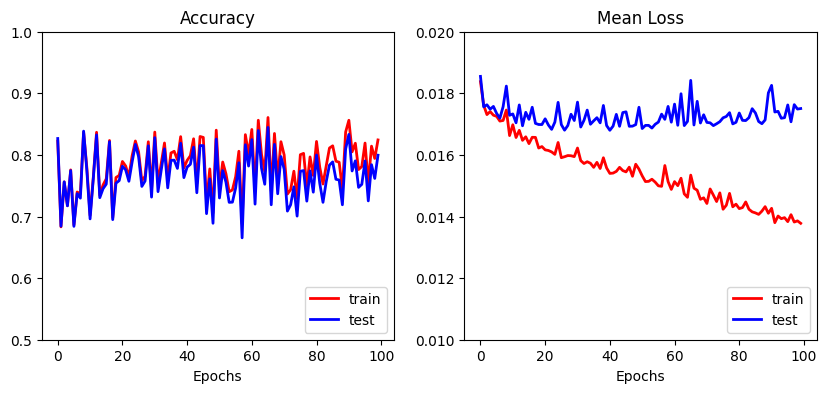
\includegraphics[width=0.8\linewidth]{eegnet_training.png}
	\captionof{figure}{Loss and accuracy at each epoch during the training of EEGNet}
	\label{fig:8}
\end{figure}

\vspace{-3mm}
As we mentioned before, it is quite necessary to balance the effect of the two classes since the target class is the absolute minority in the original dataset. Before we fix this problem, the model is trained to assign every input to the non-target class. This is intuitive since there are around $82\%$ data in the training set belonging to non-targets. Always returning the decision as the non-target class can automatically get an accuracy of $82\%$. However, the classification accuracy does not reflect the whole story. Failing to detect any target signals makes the EEGNet useless for the overall algorithmic part. After we fixed this problem, we derived a working EEGNet with the training procedure shown in Figure  \ref{fig:8}. We saved the model with the best test (validation) accuracy as the checkpoint. Although the checkpoint model is sufficient to use, we must rethink why the accuracy has such a significant fluctuation. Again, maybe only measuring the accuracy is not enough, we need to investigate other measurements, such as recall and precision.\\

\vspace{-3mm}
Now it is time to compare how well the two methods are performed on the test data. Figure \ref{fig:9} compares the signal classification accuracy. The red dotted line and blue dotted line mark the averaged accuracy for SWLDA and EEGNet correspondingly. SWLDA classifier wins by a narrow margin of $4\%$. In each method, the variation among all 13 participants is very small, so comparing the average level is enough. For the comparison of the spelling accuracy, the gap becomes more obvious, the gap not only exists between the methods but also exists among the participants. This time, the average spelling accuracy of the SWLDA-based algorithm (method 1) is around $17\%$ ahead of the EEG-based algorithm (method 2) although both are not satisfactory as both are lower than $80\%$. However, if we look at each participant's performance, we can notice that some of them have a way higher spelling accuracy than others. This observation is very important for us to interpret the results as this verifies the fact that reactions to the stimulus are very different among participants. As a result, there is no wonder that the SWLDA-based algorithm (user-specific) can perform better than the EEGNet-based algorithm (general).

\vspace{-3mm}
\begin{figure}[H]
	\centering
	\subfloat[\centering Signal classification accuracy]
	{{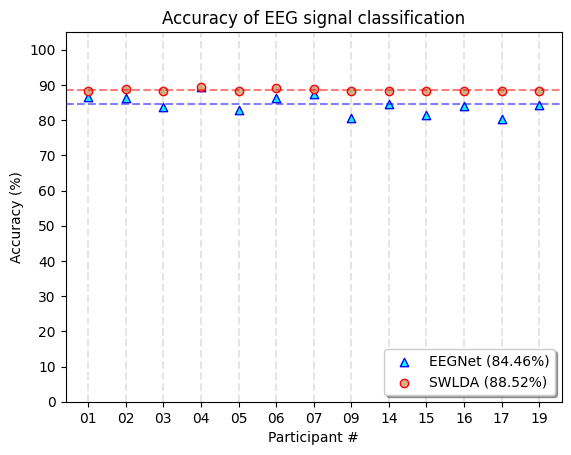
\includegraphics[width=8cm]{signal_clf_acc.png} }}%
	\qquad
	\hspace{-8mm}
	\subfloat[\centering Spelling accuracy]
	{{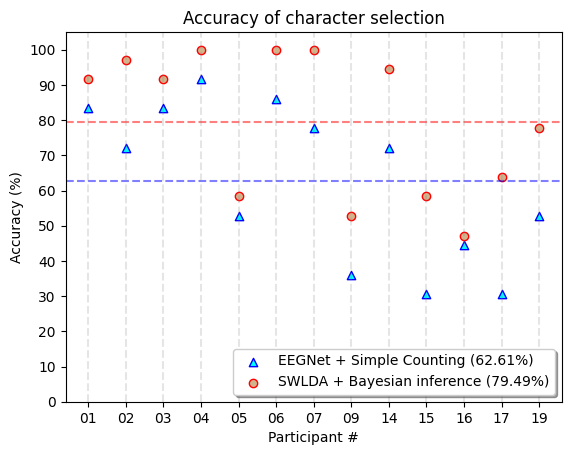
\includegraphics[width=8cm]{spelling_acc.png} }}%
	\caption{Performances of the two models on test data}
	\label{fig:9}
\end{figure}

\vspace{-3mm}
Another interesting question is: why the small gap ($4\%$) in signal classification accuracy is enlarged to $17\%$ in spelling accuracy? We believe this can be attributed to the use of the 2-gram language model and the essence of the generative probabilistic model. Firstly, when we probe into the wrong prediction made by EEGNet + simple counting, we notice that a lot of them are nearby characters around the desired one. This is a very common mistake due to the noise and the inevitable pattern that participants are prone to be distracted by the flash of the nearby characters. The 2-gram language model can eliminate this problem to some extent since it utilizes the information of the previously typed letter, which can give some initial advantage to a letter with a higher probability of being the next desired character.\\

\vspace{-3mm}
Even though the SWLDA-based algorithm seems to be the better one (after all, it remains as the state-of-the-art method for a long time till now), we should not ignore the upsides and bright potentials of the EEGNet. The biggest advantage is that it does show the generalizability across different participants. It is very likely a higher accuracy can be achieved by feeding with more data and equipping with better training setups. In fact, we should be aware that the pre-training process is very tedious for the users. If we can bypass it with a given general classifier, it will make the P300 speller more user-friendly and easy to use. Even if the original EEGNet is not good work, we can leverage transfer learning to adapt the original one to be more user-specific, which is still better than training a SWLDA classifier for each user from scratch.


\subsection{Extra 1: Evaluating the postive effect of the 2-gram LM on the P300 speller}
It is worth figuring out how much performance increment the 2-gram LM we used here can bring to the P300 speller. To know this, it is necessary to control the other variables by using the same classification algorithm (SWLDA), the same training and testing settings, and the same inference algorithm (Bayesian inference). We followed the same instructions and used the same online dataset from \cite{mainsah2014utilizing}. Note that from now we have changed to use the dynamic stopping (DS) paradigm rather than the static stopping (SS) we used before. The difference is that the DS paradigm will instantly stop the iterations whenever the algorithm is confident enough to infer the desired character. This allows the algorithm to stop earlier than the preset maximum number of flashes. To reach a certain confidence level, the algorithm usually requires the highest score among the characters to be lower than a certain threshold. For methods using Bayesian inference, this threshold can be $0.9$, which is also what we will use in this extra experiment.

\vspace{-3mm}
\begin{figure}[H]
	\centering
	\subfloat[\centering Avergage spelling accuracy]
	{{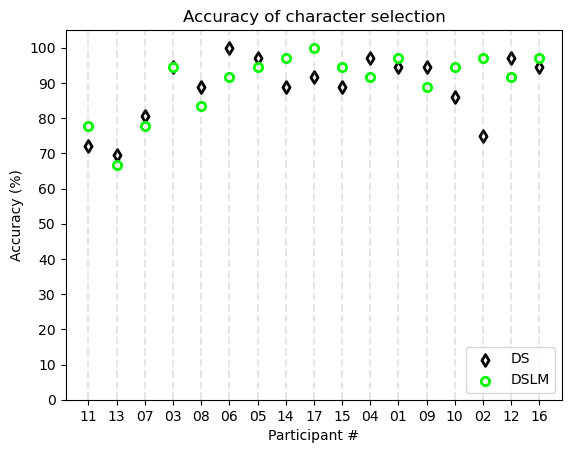
\includegraphics[width=8cm]{extra1/accuracy.png} }}%
	\qquad
	\hspace{-8mm}
	\subfloat[\centering Average required flashes/character]
	{{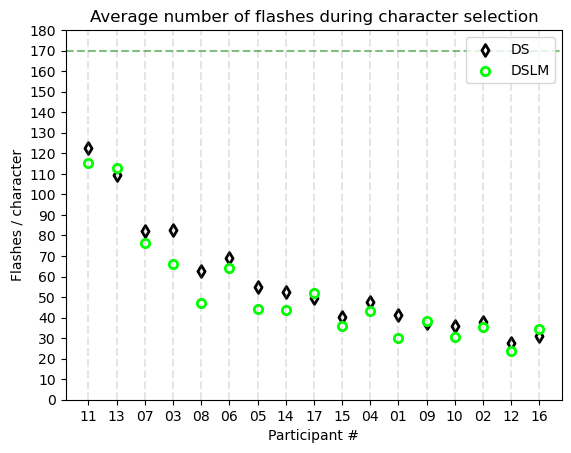
\includegraphics[width=8cm]{extra1/avg_flashes_per_char.png} }}%
	\caption{Performances of the P300 speller with and wihout the assistant of the 2-gram LM}
	\label{fig:10}
\end{figure}

\vspace{-3mm}
Figure \ref{fig:10} shows that the 2-gram LM can effectively further improve the average spelling accuracy and time-efficiency of the P300 speller, although the increment varies on different subjects. Note that the subjects here are ordered ascendingly by their detectability index, defined as how far away the distributions of classifier scores in the target class and non-target class are separated (the details are specified in \cite{mainsah2016using}). Since the detectability index is strongly correlated with the performance, this can validate the correctness of the results, and also help readers to capture more information.


\subsection{Extra 2: Improving Method 2 by using Bayesian Inference and 2-gram LM}
It is possible to integrate Bayesian Inference with the EEG-based P300 speller. Previously, we set the output of EEGNet as a vector with two elements $[a, b]$, measuring the possibility of being the target and non-target respectively. In fact, we can simply modify this output layer by converting it to a classifier score (scalar) using $\frac{e^a}{e^a + e^b}$, inspired by the softmax function. Then, the following procedures are the same as what we did in method 1 previously: the inference algorithm will use the classifier score to update the score of each character by Equation \ref{eq:1} and \ref{eq:2}, while the auxiliary 2-gram LM help to initialize the scores according to Equation \ref{eq:4}.

\vspace{-3mm}
\begin{figure}[H]
	\centering
	\subfloat[\centering Previous method 2]
	{{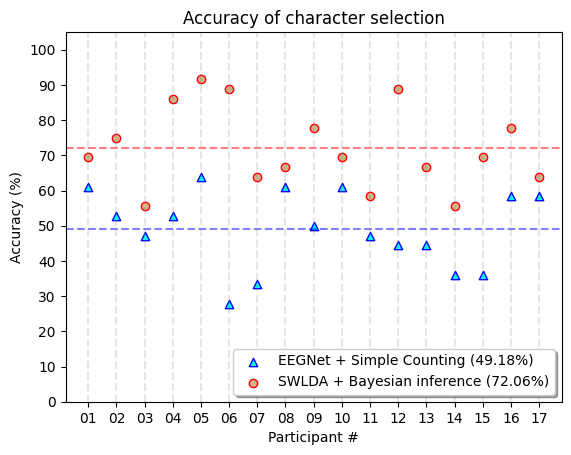
\includegraphics[width=8cm]{extra2/spelling_acc(old).png} }}%
	\qquad
	\hspace{-8mm}
	\subfloat[\centering Upgraded method 2]
	{{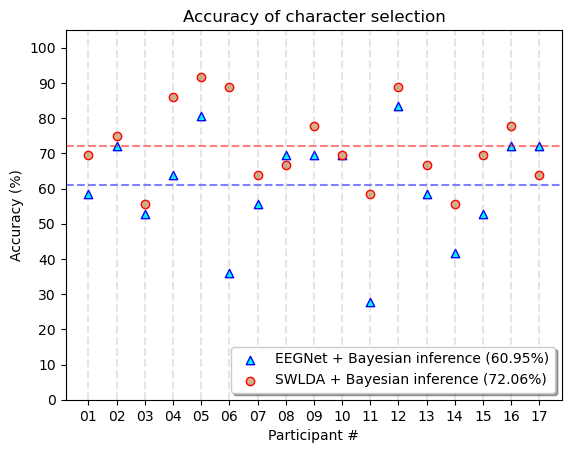
\includegraphics[width=8cm]{extra2/spelling_acc.png} }}%
	\caption{Performances of the upgraded method 2 (with Bayesian inference and 2-gram LM)}
	\label{fig:11}
\end{figure}

\vspace{-3mm}
This time, the gap in spelling accuracy between method 1 and method 2 is narrowed to $12\%$ compared with $24\%$ before upgrading. This is inspiring as it brings the visible hope that EEGNet-based solution can be further improved to get a competitive performance close to the SWLDA-based method, while still preserving the strong generalizability.



\section{Conclusion} \label{Conclusion}
\vspace{-3mm}
In this study, we successfully implemented two representative but completely different solutions in P300 spellers. Method 1 (SWLDA-based) represents the "old-school" side of traditional machine learning, whereas method 2 (EEGNet classifier and simple counting) represents the new trend of deep learning, seeking to achieve generalizability. By comparing their performance on real data, the SWLDA-based method defends its title as the state-of-the-art solution, but we should not forget that the language model we added to it also enhances its performance. On the other hand, the result that the EEG-based method fell behind doesn't hide its value and potential. We have to admit that we didn't maximize the power of this deep neural network as the training setup is not optimized, but this also reflects how promising if it can be improved with more data and better training configuration since it already shows a convincing sign of generalizability.\\

\vspace{-3mm}
Personally, I learned a lot from this semester-long independent study. The implementation of many algorithms undoubtedly enhances my coding skills, but more importantly, consolidates my comprehension of the techniques. If reading high-quality papers can gain half of the knowledge, then translating the idea to code and conducting the experiments are the necessary conditions to finish the remaining half.\\

\vspace{-3mm}
Speaking of future work, the key goal is to keep updating the EEGNet until it is good enough to challenge the title of "state-of-the-art". To further validate EEGNet's generalizability, we should test it on some unseen subjects rather than just unseen data from the same group of subjects. Furthermore, with the booming development of natural language processing (NLP), it could be very interesting to find some latest techniques in NLP that are suitable for the P300 spellers.

\bibliographystyle{unsrtnat}
{\small \bibliography{references}}
\end{document}
